\chapter{De Methodo Orationis Mentalis Dom Vitalis Lehodey}
\begin{center}
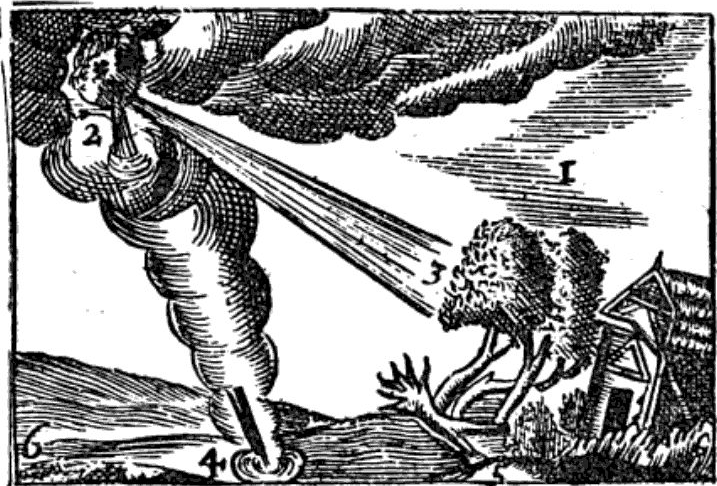
\includegraphics[scale=0.5]{Air.png}
\end{center}

\section{Intended Audience}
This is intended for students who have completed Lectio 7 and 8 of Latin by the Natural Method and Chapter 6 of Lingua Latina Per Se Illustrata. There are 533 words in this chapter.

\section{Text}
In silvā Jēremīās et Eliseus ambulāvērunt. Jēremīās dīxit ad Eliseum "Unde vēnistī\footnote{\textbf{} = You come}?". "Nātus sum\footnote{\textbf{} = I was born} in Britanniā, ubi sumus?". "In Ītaliā sumus\footnote{\textbf{} = We are}. Nōn Rōmae, nōn Tusculī, nōn Tarentīī, sed in Ītaliā." Jēremīās respondit. "Unde vēnistī?" interrogāvit Eliseus. "Isrāēl est ubi nātus sum, ante Chrīstum nātum, sed nātus es post Chrīstum nātum?". "Sum, duo mīlia\footnote{\textbf{} = Thousands} annī post Chrīstum nātum.". Aura\footnote{\textbf{} = Breeze} bona flabat\footnote{\textbf{} = It blew} per arborēs, et placebat\footnote{\textbf{} = It was pleasing} Jēremīae\footnote{\textbf{} = To Jeremiah} et Eliseo\footnote{\textbf{} = To Elisha}. "Bona aura est In Silvā, flantur arborēs.  Quō vēnerit?" ait Eliseus. Respondit "Nesciō. Deus scit, et scīvit ante creātiōnem\footnote{\textbf{} = Creation} mundī". "Sīcut Deus spīrat\footnote{\textbf{} = He breathes} super\footnote{\textbf{} = Over} nōs.  Bene flat haec aura. Ignis nōn tam bonus est quam aura." ait Eliseus. "Quid? nōn placet tibi ignis meus? Aura tam bona nōn est quam ignis. Haec frīgida\footnote{\textbf{} = Cold} aura nōn tam calida\footnote{\textbf{} = Hot} est quam ignis." respondit Jēremīās. "Vetus\footnote{\textbf{} = Old} vir!" exclāmāvit Eliseus "Senectūs\footnote{\textbf{} = Old Age} tua cēpit laetitiam bonae aurae ex tē". "Cēpit" respondit "Nōlī exclāmāre dē hāc rē\footnote{\textbf{} = Don't shout about this thing}". "Sed" Jēremīās addidit\footnote{\textbf{} = He added} "nōn cēpit Ventus\footnote{\textbf{} = Wind} Deī, flat in corde meō". 

"Quid est hic ventus?" interrogāvit Eliseus. "Ventus, vel ignis ōrātiōnis meae quī spīrat in mē". "Ignis? Quid ignis?". "Ignis ōrātiōnis mentālis\footnote{\textbf{} = The Fire of Mental Prayer}" respondit "Quī īnstrūxit\footnote{\textbf{} = It taught me} mē in amōre et virtūte, Ventus cognitiōnis\footnote{\textbf{} = Experience, Intuitive Knowledge} Deī, nōn sīcut scientia\footnote{\textbf{} = Intellectual Knowledge in the sense of book learning} theologiae\footnote{\textbf{} = Of theology}". "Quōmodo habeō cognitiōnem Deī? Volō habēre\footnote{\textbf{} = I want to have} procellam\footnote{\textbf{} = Gust, Gale (In some contexts, storm) } Cognitiōnis Deī.". "Procella? Cūr interrogāvistī rem parvam? Cūr nōn interrogāvistī turbinem\footnote{\textbf{} = Tornado, Whirlwind}? Deus appāruit Moȳsī in Aegyptō, et fuit in turbine flammae. Haec turbō dūxit\footnote{\textbf{} = It led} populum eius ex Aegyptō. Cūr procellam sōlam\footnote{\textbf{} = Alone} interrogāvistī? Deus amat\footnote{\textbf{} = He loves} eum quī vult meliōrem\footnote{\textbf{} = Better} amōrem.". "Quōmodo possum facere\footnote{\textbf{} = How can I make} ōrātiōnem mentālem?" interrogāvit. 

"Dīcam\footnote{\textbf{} = I will speak} dē methodō\footnote{\textbf{} = Method} Dom Vītālīs Lehoedy. Scrīpsit\footnote{\textbf{} = He wrote} librum\footnote{\textbf{} = Book}." respondit Jēremīās. "Prīmō, Franciscus Salensius Sānctus dīxit facere ūnam hōram\footnote{\textbf{} = Hour} ōrātiōnis mentālī in diē ūnā. Lehodey (quī scrīpsit viās ōrātiōnis mentālis (Ways of Mental Prayer anglice), quem auscultās\footnote{\textbf{} = You are listening}, dīxit facere dīmidiam\footnote{\textbf{} = Half} partem\footnote{\textbf{} = Part} hōrae. Potes loquī\footnote{\textbf{} = You can speak} cum presbytērō dē tempore\footnote{\textbf{} = Time} ōrātiōnis mentālis. ". "Deinde?" respondit Eliseus. "Tolle\footnote{\textbf{} = Take!} librum, quī est dē vitiīs\footnote{\textbf{} = Vices}, vel dē virtūtibus\footnote{\textbf{} = Virtues}, vel dē mystēriīs Fideī\footnote{\textbf{} = Mysteries of Faith}. Quīcumque\footnote{\textbf{} = Whatever} bonus est tibi. Liber quem Lehodey dīxit bonum appēllātur\footnote{\textbf{} = It is called} "Preparation For Death" vel praeparātiō mortis, quae scrīptus est ā Sānctō Alphonsō ā Ligōriō". "Deinde" perrēxit\footnote{\textbf{} = He continued} Jēremīās "Tolle pāginam, et lege\footnote{\textbf{} = Read!} eam quater\footnote{\textbf{} = Four times}. Fac\footnote{\textbf{} = Do! Make!} hanc rem quia in mente dēbeō habēre pāginam.". "Sīcut dīxit Dāvīd in Psalmō\footnote{\textbf{} = Psalm} Prīmō, "Beātus vir quī meditābitur\footnote{\textbf{} = He will meditate} in lēge\footnote{\textbf{} = Law} suā diē\footnote{\textbf{} = Day} ac\footnote{\textbf{} = and} nocte\footnote{\textbf{} = Night}."" dīxit Eliseus. "Bene dīxistī, Elisee, in hōc modō meditārī possumus\footnote{\textbf{} = In this way we can meditate}". "Deinde, cōgitā\footnote{\textbf{} = Think!} dē hāc rē in pāginā est. Fortasse\footnote{\textbf{} = Perhaps}, dē patientiā\footnote{\textbf{} = Patience} Chrīstī in cruce, vel dē lēge novā\footnote{\textbf{} = New}. Cōgitā\footnote{\textbf{} = Think!} "Quōmodo possum\footnote{\textbf{} = I can} facere praecepta\footnote{\textbf{} = Commandments} Dominī?" vel\footnote{\textbf{} = Or} "Quōmodo possum dīligere Deum sīcut is dīligit mē?". "Intellegō" respondit Eliseus. "Deinde, ex cōnsīderātiōne hāc, ōra ad Deum. Cōnsīderātiō\footnote{\textbf{} = Consideration} nōn est ōrātiō, sed cōnsīderātiō dat auxilium\footnote{\textbf{} = Help} ōrātiōnī\footnote{\textbf{} = To prayer}. Dīc\footnote{\textbf{} = Say!} Deō dē cōnsīderātiōne, in precibus\footnote{\textbf{} = In prayers} interrogā grātiās\footnote{\textbf{} = Graces} ex eō. Postrēmō\footnote{\textbf{} = Finally}, fac resolūtiōnem\footnote{\textbf{} = Resolution} ex precibus et ex cōnsīderātiōne. Dīc Deō "Fēcerō\footnote{\textbf{} = I will do, I will make} hanc rem, quam facere necesse est.". 

Subitō\footnote{\textbf{} = Suddenly}, Procella flāvit, et arborēs sternēbantur\footnote{\textbf{} = They were being stretched out}. Procella sternēbat\footnote{\textbf{} = It stretched out} arborēs. Foenum\footnote{\textbf{} = Grass} etiam sternēbātur ā procellā. . Arbor cecīdit\footnote{\textbf{} = It fell} inter\footnote{\textbf{} = Between} Jēremīam et Eliseum. Cecidērunt in terrā. "Bene valēsne?" Eliseus interrogāvit. "Valeō" respondit Jēremīās.  Deinde, terra movet sē. "Quid, iam terraemōtus\footnote{\textbf{} = Earthquake}?". "In temporibus antīquīs\footnote{\textbf{} = Ancient}, cōgitābant quod Terraemōtus accidit\footnote{\textbf{} = It happened} quia ventī subterrāneī\footnote{\textbf{} = Underground} flant, et terra movētur ā hīs\footnote{\textbf{} = These} ventīs. Jēremīās surrēxit\footnote{\textbf{} = He rose} et extendit\footnote{\textbf{} = He extended} manum suam "Vēnī mēcum". Jēremīās cēpit manum Elisēī et trāxit\footnote{\textbf{} = He dragged} eam. Eliseus stetit\footnote{\textbf{} = He stood}, deinde ambulāvērunt in silvam.